\documentclass{beamer}
\mode<presentation>
\usepackage{amsmath,amssymb,mathtools}
\usepackage{textcomp}
\usepackage{gensymb}
\usepackage{adjustbox}
\usepackage{subcaption}
\usepackage{enumitem}
\usepackage{multicol}
\usepackage{listings}
\usepackage{url}
\usepackage{graphicx} % <-- needed for images
\def\UrlBreaks{\do\/\do-}

\usetheme{Boadilla}
\usecolortheme{lily}
\setbeamertemplate{footline}{
  \leavevmode%
  \hbox{%
  \begin{beamercolorbox}[wd=\paperwidth,ht=2ex,dp=1ex,right]{author in head/foot}%
    \insertframenumber{} / \inserttotalframenumber\hspace*{2ex}
  \end{beamercolorbox}}%
  \vskip0pt%
}
\setbeamertemplate{navigation symbols}{}

\lstset{
  frame=single,
  breaklines=true,
  columns=fullflexible,
  basicstyle=\ttfamily\tiny   % tiny font so code fits
}

\numberwithin{equation}{section}

% ---- your macros ----
\providecommand{\nCr}[2]{\,^{#1}C_{#2}}
\providecommand{\nPr}[2]{\,^{#1}P_{#2}}
\providecommand{\mbf}{\mathbf}
\providecommand{\pr}[1]{\ensuremath{\Pr\left(#1\right)}}
\providecommand{\qfunc}[1]{\ensuremath{Q\left(#1\right)}}
\providecommand{\sbrak}[1]{\ensuremath{{}\left[#1\right]}}
\providecommand{\lsbrak}[1]{\ensuremath{{}\left[#1\right.}}
\providecommand{\rsbrak}[1]{\ensuremath{\left.#1\right]}}
\providecommand{\brak}[1]{\ensuremath{\left(#1\right)}}
\providecommand{\lbrak}[1]{\ensuremath{\left(#1\right.}}
\providecommand{\rbrak}[1]{\ensuremath{\left.#1\right)}}
\providecommand{\cbrak}[1]{\ensuremath{\left\{#1\right\}}}
\providecommand{\lcbrak}[1]{\ensuremath{\left\{#1\right.}}
\providecommand{\rcbrak}[1]{\ensuremath{\left.#1\right\}}}
\theoremstyle{remark}
\newtheorem{rem}{Remark}
\newcommand{\sgn}{\mathop{\mathrm{sgn}}}
\providecommand{\abs}[1]{\left\vert#1\right\vert}
\providecommand{\res}[1]{\Res\displaylimits_{#1}}
\providecommand{\norm}[1]{\lVert#1\rVert}
\providecommand{\mtx}[1]{\mathbf{#1}}
\providecommand{\mean}[1]{E\left[ #1 \right]}
\providecommand{\fourier}{\overset{\mathcal{F}}{ \rightleftharpoons}}
\providecommand{\system}{\overset{\mathcal{H}}{ \longleftrightarrow}}
\providecommand{\dec}[2]{\ensuremath{\overset{#1}{\underset{#2}{\gtrless}}}}
\newcommand{\myvec}[1]{\ensuremath{\begin{pmatrix}#1\end{pmatrix}}}
\let\vec\mathbf

\title{Matgeo Presentation - Problem 9.7.7}
\author{ee25btech11063 - Vejith}

\begin{document}


\frame{\titlepage}
\begin{frame}{Question}
\text{Find the solution of the pair of equations:} \quad 
$\frac{3}{x} + \frac{8}{y} = -1, 
\qquad 
\frac{1}{x} - \frac{2}{y} = 2, 
\qquad x,y \neq 0.$
\end{frame}

\begin{frame}{Solution}
    let 
\begin{align}
    \frac{1}{x}=u\\
    \frac{1}{y}=v\\
    \implies 3u+8v=-1\\
    u-2v=2
\end{align}
Equations (0.3) and (0.4) cann be written as
\begin{align}
    \begin{pmatrix}
        3 & 8\\
        1 & -2
    \end{pmatrix}\myvec{u\\v}=\myvec{-1\\2}
\end{align}
Forming the augmented matrix
\begin{align}
    \implies 
\left(\begin{array}{cc|c}
        3 & 8 & -1 \\
        1 & -2 & 2 
\end{array}\right) 
\xleftrightarrow{R_2 \rightarrow R_2-\frac{1}{3} \times R_1} \left(\begin{array}{cc|c}
        3 & 8 & -1 \\
        0 & -\frac{14}{3} & \frac{7}{3} 
\end{array}\right) 
\end{align}
\end{frame}

\begin{frame}{Conclusion}
on back substitution we get 
\begin{align}
    \myvec{u\\v}=\myvec{1\\-\frac{1}{2}}
\end{align}
From (0.1) and (0.2) we get
\begin{align}
    \myvec{x\\y}=\myvec{1\\-2}
\end{align}
\end{frame}

\begin{frame}{Plot}
    \begin{figure}
    \centering
    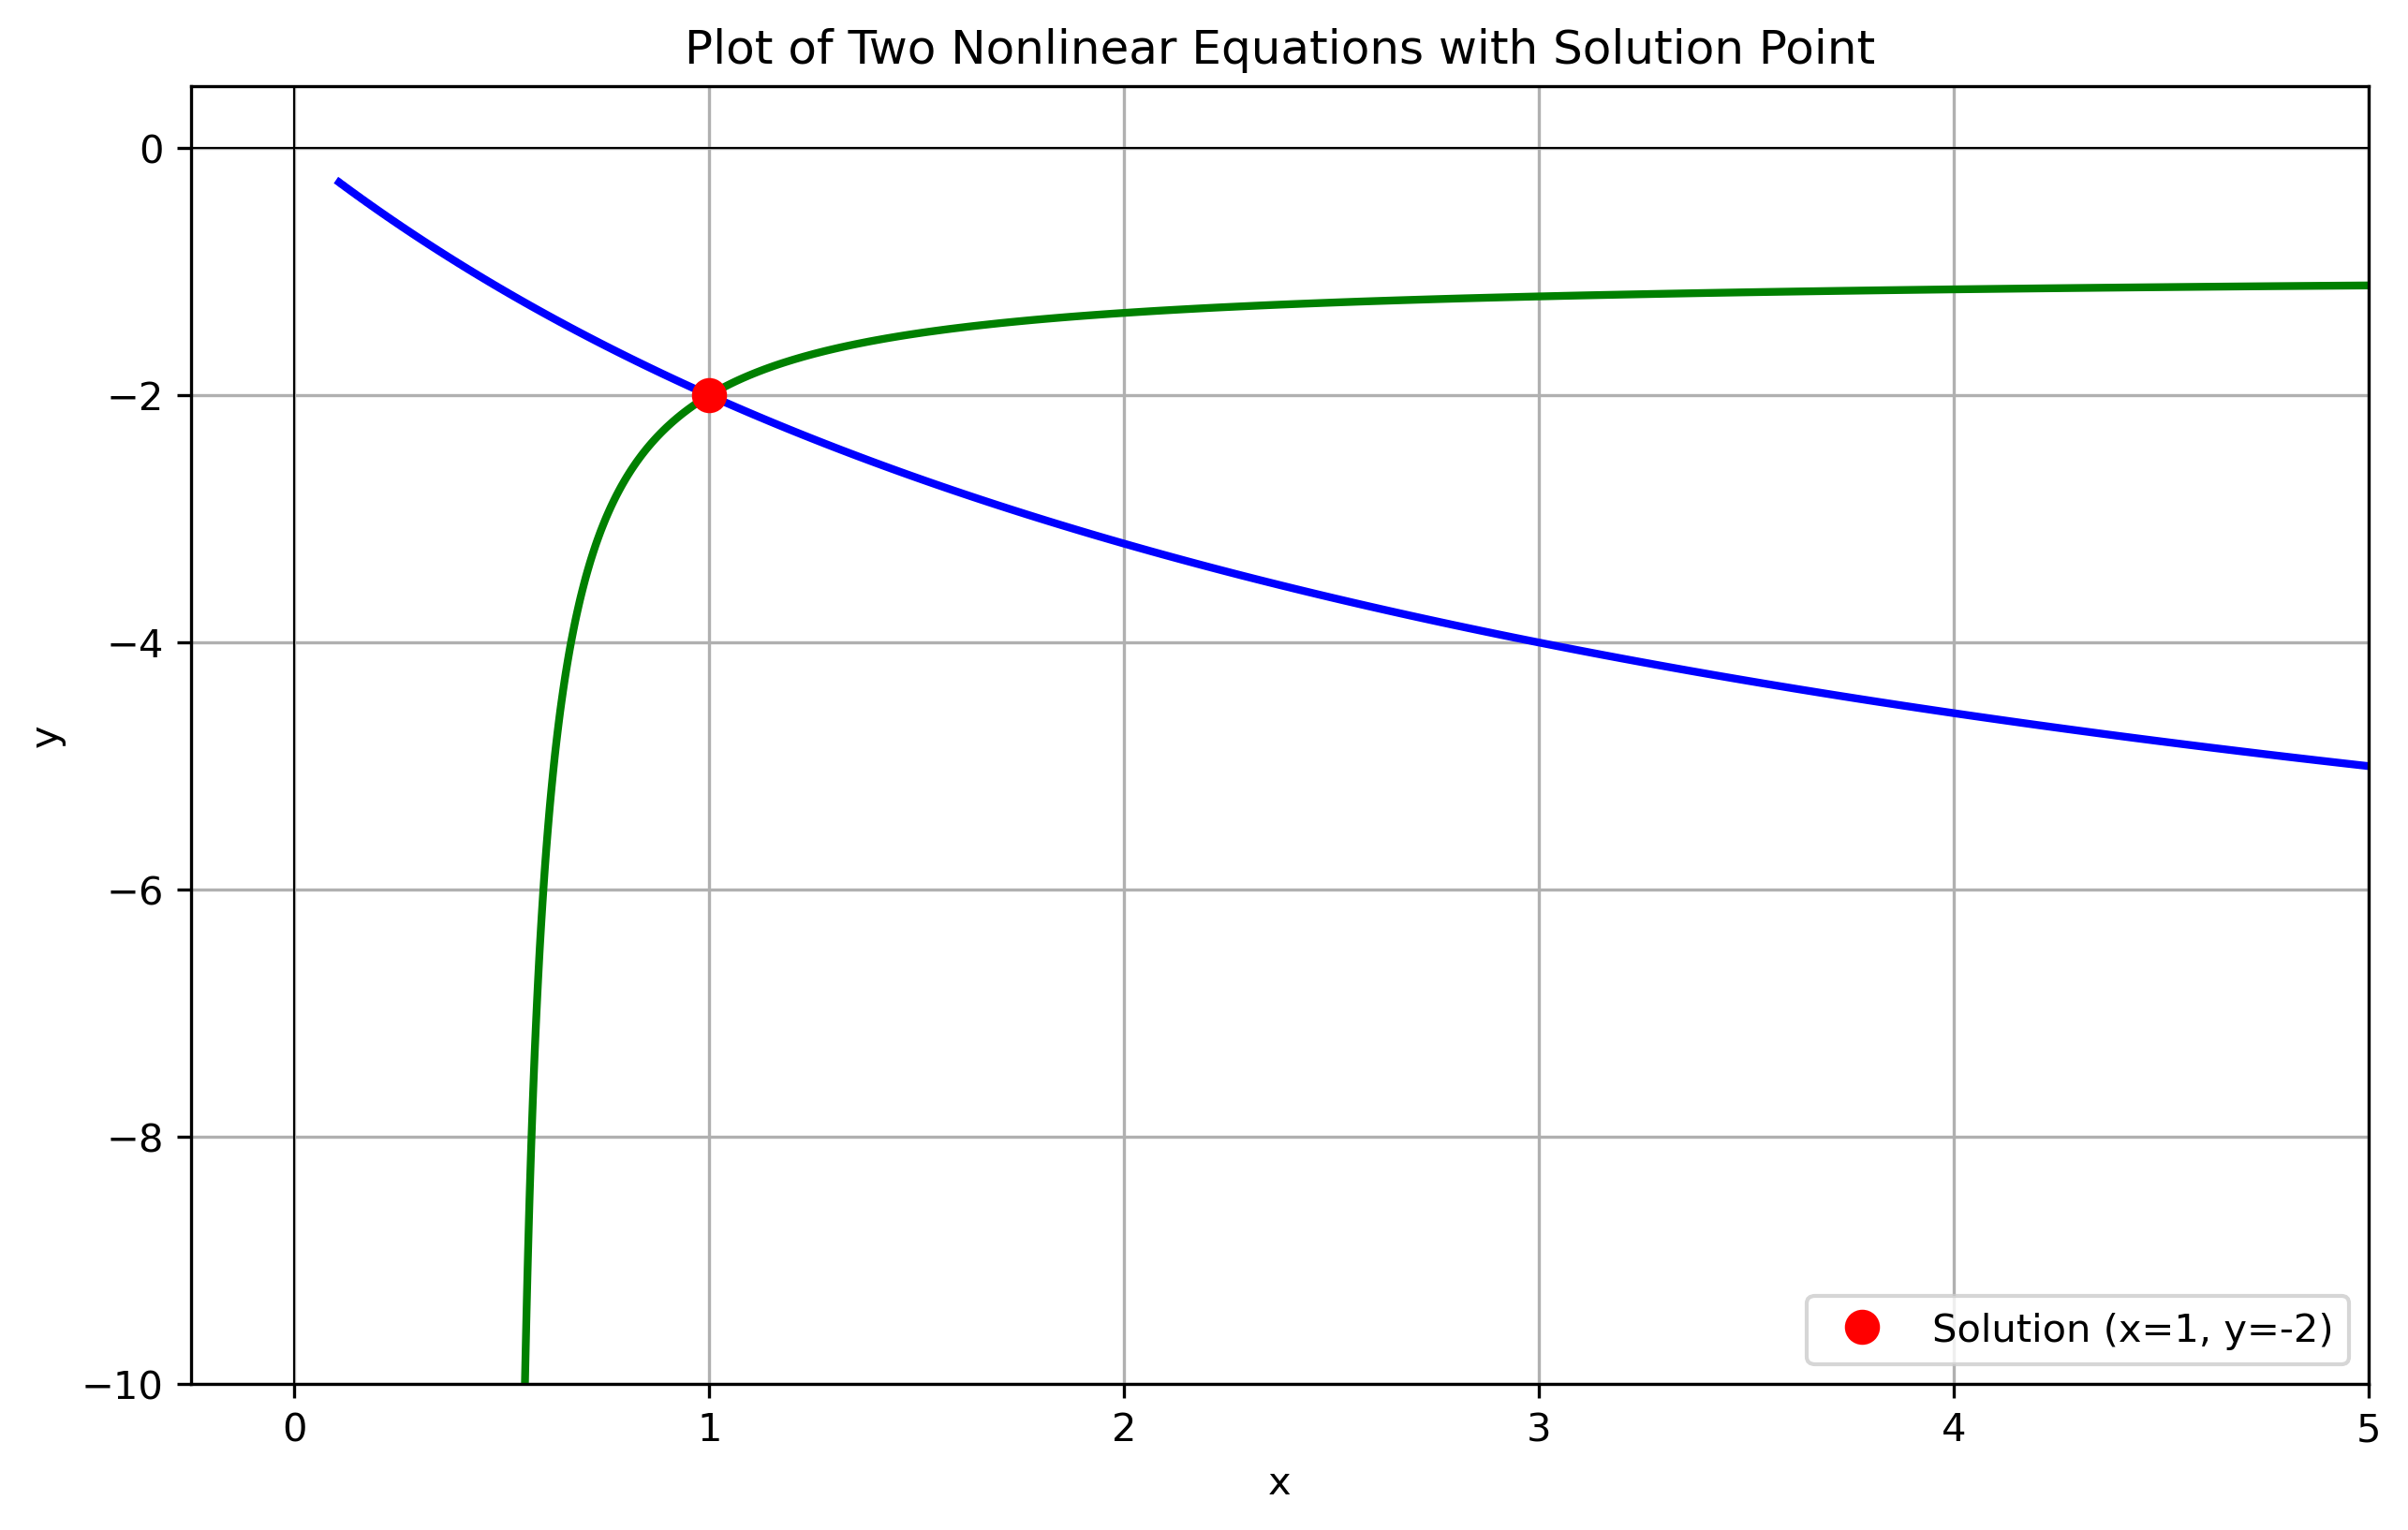
\includegraphics[width=0.85\columnwidth]{figs/01.png}
    \caption{}
    \label{fig:placeholder}
\end{figure}
\end{frame}

% --------- CODE APPENDIX ---------
\section*{Appendix: Code}

% C program
\begin{frame}[fragile]{C Code: area.c}
\begin{lstlisting}[language=C]
#include <stdio.h>

int main() {
    FILE *fp;
    double u, v, x, y;

    // Open file for writing (including status and solution)
    fp = fopen("answer.dat", "w");

    if (fp == NULL) {
        return 1;  // Cannot proceed if file can't be opened
    }

    // Check for division by zero
    if (u == 0.0 || v == 0.0) {
        fprintf(fp, "Error: Division by zero encountered while computing x or y.\n");
        fclose(fp);
        return 1;
    }

    // Compute x and y
    x = 1.0 / u;  // x = 1.0
    y = 1.0 / v;  // y = -2.0

    // Write the solution to file
    fprintf(fp, "The solution is:\n");
    fprintf(fp, "x = %.2lf\n", x);
    fprintf(fp, "y = %.2lf\n", y);

    fclose(fp);
    return 0;
}


\end{lstlisting}
\end{frame}

% Python plotting
\begin{frame}[fragile]{Python: plot.py}
\begin{lstlisting}[language=Python]
import numpy as np
import matplotlib.pyplot as plt

# Solution point from algebra
x_sol = 1
y_sol = -2

# Define ranges, avoiding x=0 and y=0
x_vals = np.linspace(0.1, 5, 400)
y_vals = np.linspace(-10, -0.1, 400)

# Create meshgrid
X, Y = np.meshgrid(x_vals, y_vals)

# Define the equations:
# 1. (3/x + 8/y + 1 = 0)
# 2. (1/x - 2/y - 2 = 0)
eq1 = (3 / X) + (8 / Y) + 1
eq2 = (1 / X) - (2 / Y) - 2

# Plot
plt.figure(figsize=(10, 6))

# Contour where each equation is zero
plt.contour(X, Y, eq1, levels=[0], colors='blue', linewidths=2, linestyles='solid')
plt.contour(X, Y, eq2, levels=[0], colors='green', linewidths=2, linestyles='solid')

# Plot point of intersection
plt.plot(x_sol, y_sol, 'ro', markersize=8, label=f'Solution (x={x_sol}, y={y_sol})')

# Labels and styling
plt.title('Plot of Two Nonlinear Equations with Solution Point')
plt.xlabel('x')
\end{lstlisting}
\end{frame}

\begin{frame}[fragile]{Python: plot.py}
\begin{lstlisting}[language=Python]
plt.ylabel('y')
plt.axhline(0, color='black', lw=0.5)
plt.axvline(0, color='black', lw=0.5)
plt.grid(True)
plt.legend()

# Save the plot
plt.savefig("equation_plot.png", dpi=300, bbox_inches='tight')
plt.close()  # Close the figure to avoid showing it if not needed

print("Plot saved as 'equation_plot.png'")


\end{lstlisting}
\end{frame}
\end{document}
